\documentclass[../sparc.tex]{subfiles}
\graphicspath{{\subfix{../images/}}}
\begin{document}

%%%%%%%%%%%%%%%%%%%%%%%%%%%%%%%%%%%%%%%%%%%%%%%%%%%%%%%%%%%%%%%%%%%%%%%%%%%%%%%%
\section{Длина волны}

При создании ``мигающего светодиода'' мы попеременно подавали на цифровой порт
сигналы \texttt{HIGH} и \texttt{LOW}, с указанием задержки (в миллисекундах.)
Если мы посмотрим на вид сигнала на цифровом порту во времени (скажем, с помощью
осциллографа), то увидим график, примерно как на
рис. \ref{fig:blinking-led-graph}.  Где \emph{длительность периода} -- расстояние
между двумя ближайшими друг к другу точками в пространстве, в которых колебания
происходят в одинаковой фазе.

\begin{figure}[ht]
  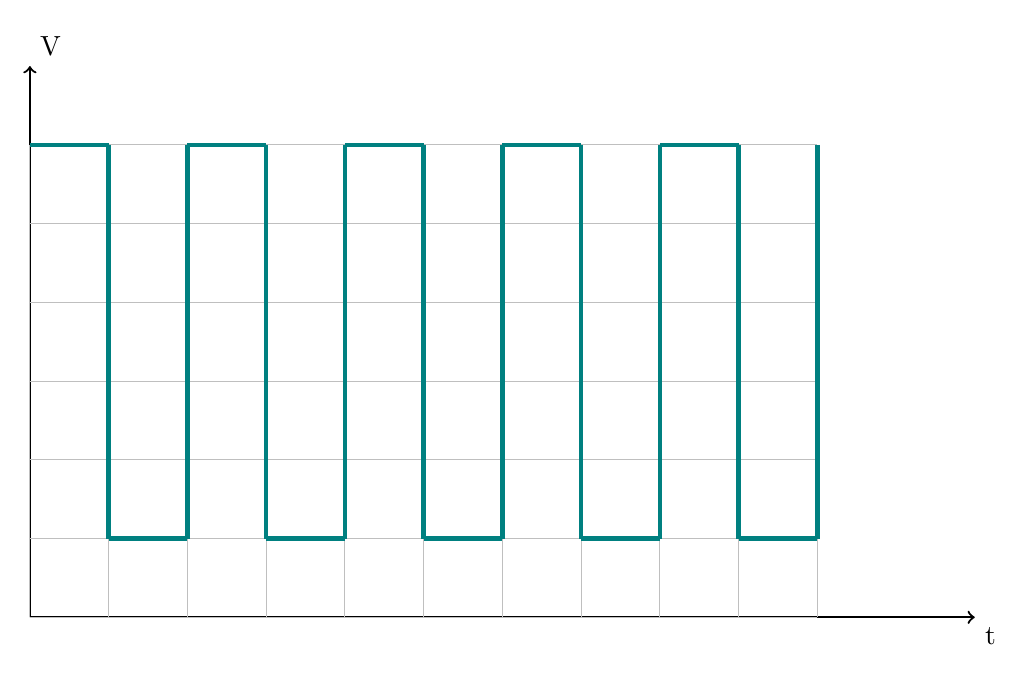
\begin{tikzpicture}
    \draw[thick, ->] (0, 0) -- (12, 0) node[anchor=north west] {t};
    \draw[thick, ->] (0, 0) -- (0,  7) node[anchor=south west] {V};
    \draw[lightgray] (0, 0) grid (10, 6);
    \foreach \x in {0, 2, ..., 8} {
      \draw[ultra thick, teal] (\x, 6) -- (\x + 1, 6);
      \draw[ultra thick, teal] (\x + 1, 6) -- (\x + 1, 1);
      \draw[ultra thick, teal] (\x + 1, 1) -- (\x + 2, 1);
      \draw[ultra thick, teal] (\x + 2, 1) -- (\x + 2, 6);
    }
  \end{tikzpicture}
  \caption{Графическое отображение сигнала, меняющегося во времени, на цифровом
    порту.}
  \label{fig:blinking-led-graph}
\end{figure}

Зная длительность периода, можно рассчитать \emph{частоту колебаний}, и наоборот
-- зная частоту, можно рассчитать длину волны.

При работе с \gls{ШИМ} мы будем использовать длительность периода, заданную в
микросекундах (мкс.)  1 микросекунда -- это одна миллионная часть секунды. Для
краткости записи подобных маленьких величин часто используется возведение числа
10 в отрицательную степень.  Ниже приведена таблица \ref{table:timescale-units}
с указанием различных долей секунды. \footnote{Для полного списка кратных и
дольных единиц см. статью
\href{https://ru.wikipedia.org/wiki/\%D0\%A1\%D0\%B5\%D0\%BA\%D1\%83\%D0\%BD\%D0\%B4\%D0\%B0}{Секунда}
в Википедии.}

\begin{table}[H]
  \begin{tabular}{p{3cm}|p{4cm}|p{3cm}}
    Название & Величина & Пример \\
    \hline \hline
    секунда (с) & $ 1 \mbox{с} $ или $ 10^0 \mbox{с} $ & $ 500 * 10^{0} = 500 \mbox{с} $ \\
    \hline
    миллисекунда (мс) & $ 0.001 \mbox{c} $ или $ 10^{-3} \mbox{c} $ & $ 500 * 10^{-3} = 500 \mbox{мс} $ \\
    \hline
    микросекунда (мкс) & $ 0.000001 \mbox{c} $ или $ 10^{-6} \mbox{c} $ & $ 500 * 10^{-6} = 500 \mbox{мкс} $ \\
    \hline
    наносекунда (нс) & $ 0.000000001 \mbox{c} $ или $ 10^{-9} \mbox{с} $ & $ 500 * 10^{-9} = 500 \mbox{нс} $
  \end{tabular}
  \caption{Единицы измерения времени.}
  \label{table:timescale-units}
\end{table}

\end{document}
